\section{Visual Studio Projektmappe}

Das gesamte Projekt befindet sich in einer Visual Studio Projektmappe, welch in folgene Unterprojekte gegliedert ist:
\begin{itemize}
    \item \textbf{Common.Dal.Ado}: Hier befinden sich Hilfsklassen, die den Umgang mit ADO.NET leichter gstalten.
    \item \textbf{Wetr.Domain}: Dieses Projekt beinhaltet die Domainobjekte, welche als einfache Datenbehälter genutzt werden.
    \item \textbf{Wetr.Dal.Interface}: In diesem Paket befinden sich die Interfaces für die Datenzugriffschricht für jedes Domainobjekt bzw. Tabelle.
    \item \textbf{Wetr.Dal.Ado}: Die ADO.NET Implementierung der Datenzugriffsschicht Interfaces.
    \item \textbf{Wetr.Dal.Factory} Beinhaltet Factories um die Instanziierung der benötigen komkreten Klassen zu abstrahieren.
    \item \textbf{Wetr.Test.Dal} Dieses Projekt beinhaltet Unit-Tests für die Datenzugriffsschicht.
    \item \textbf{Wetr.Generator}: Zuständig für das Generieren von Messdaten für die einzelnen Stationen.
\end{itemize}

\newpage
\subsection{Common.Dal.Ado}
Das \textit{Common.Dal.Ado} Projekt verwendet die Klassen \textit{AdoTemplate}, \textit{DefaultConnectionFactory}, \textit{IConnectionFactory}, \textit{Parameter} und  \textit{RowMapper}. In der  \textit{AdoTemplate} Klasse werden alle anderen Klassen verwendet. Mithilfe  \textit{IConnection} wird eine Verbindung zu Datenbank aufgebaut.  \textit{AdoTemplate} stellt eine Funktion  \textit{QueryAsync} bereit um eine Datenbankabfragen durchführen zu können.

\begin{figure}[H]
\centering
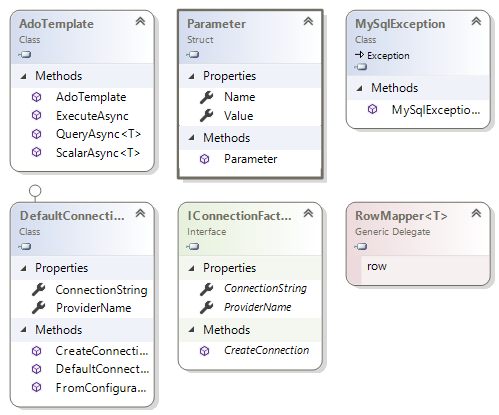
\includegraphics[width=.45\textwidth]{pictures/Common_Dal_Ado_ClassDiagramm.png}
\caption{Common.Dal.Ado UML Diagramm}
\label{fig:common.dal.ado}
\end{figure}
\raggedright

\newpage
\subsection{Wetr.Dal.Interface}
Im \textit{Wetr.Dal.Interface} Projekt wird für jede Klasse in  \textit{Wetr.Domain} ein eigenes Interface bereitgestellt das von den jeweiligen \textit{Dao} Objekten implementiert wird. Jedes Interface implementiert \textit{IDaoBase}$<$\textit{T}$>$. Dieses Interface fasst die Methoden, die in jedem abgeleiteten \textit{Dao Objekt} implementiert werden müssen, zusammen (FindAll, FindById, Delete, Insert, Update).

\begin{figure}[H]
\centering
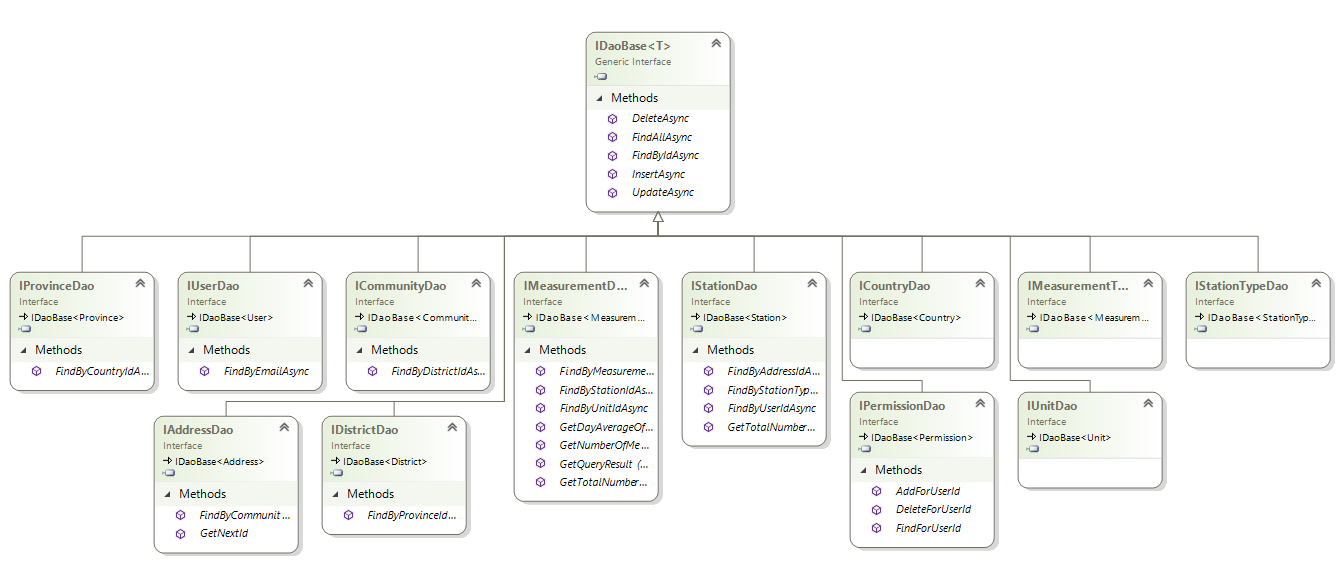
\includegraphics[width=.8\textwidth]{pictures/Wetr_Dal_Interface.png}
\caption{Wetr.Dal.Interface UML Diagramm}
\label{fig:Wetr.Dal.Interface}
\end{figure}
\raggedright

\newpage
\subsection{Wetr.Dal.Ado}
Mit den Klassen im \textit{Wetr.Dal.Ado} Projekt kann eine Verbindung zur Datenbank aufgebaut werden und spezielle SQL Operationen ausgeführt werden. Für jedes \textit{Dao} Objekt gibt es eine \textit{Wetr.Domänen} Klasse. Diese Klassen werden als Behälter Klassen für die angefragten Daten der Datenbank verwendet.

\begin{figure}[H]
\centering
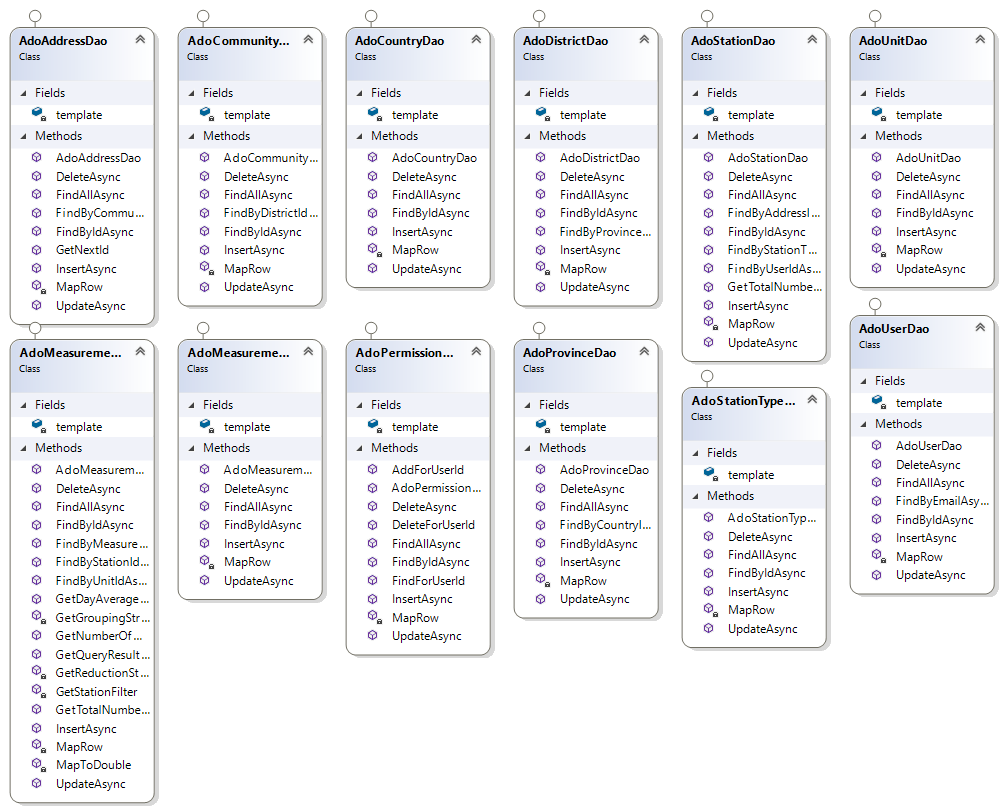
\includegraphics[width=.8\textwidth]{pictures/Wetr_Dal_Ado.png}
\caption{Wetr.Dal.Ado UML Diagramm}
\label{fig:Wetr.Dal.Ado}
\end{figure}
\raggedright

\subsection{Wetr.Dal.Factory}
Im \textit{Wetr.Dal.Factory} Projekt wird eine Klasse \textit{AdoFactory} bereitgestellt mit deren Hilfe ein \textit{Dao} Objekt erstellt werden kann.

\begin{figure}[H]
\centering
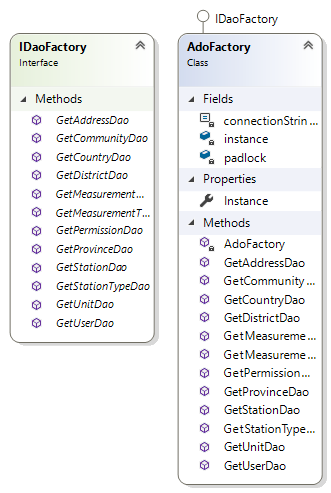
\includegraphics[width=.45\textwidth]{pictures/Wetr_Dal_Factory.png}
\caption{Wetr.Dal.Factory UML Diagramm}
\label{fig:Wetr.Dal.Factory}
\end{figure}
\raggedright

\newpage
\subsection{Wetr.Domain}
Das \textit{Wetr.Domain} Projekt enthält alle Behälterklassen für alle \textit{Dao} Objekte.

\begin{figure}[H]
\centering
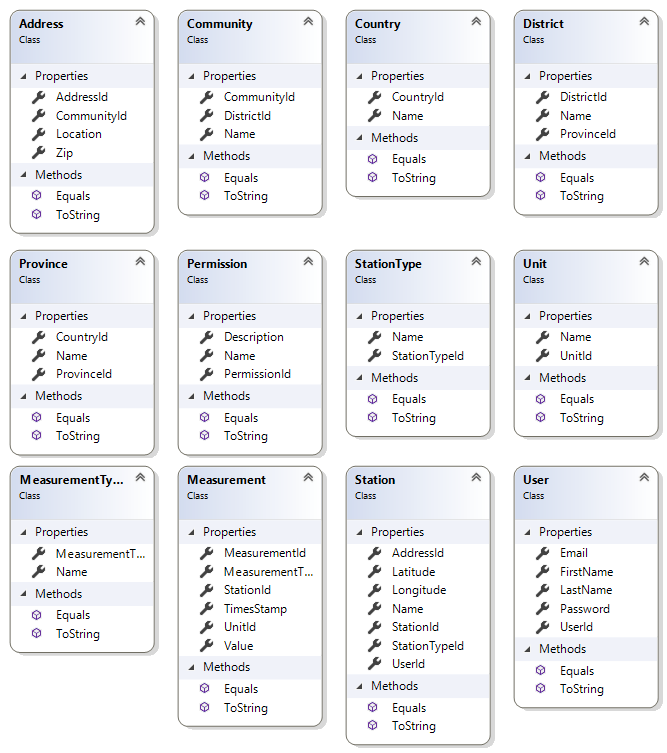
\includegraphics[width=.8\textwidth]{pictures/Wetr_Domain.png}
\caption{Wetr.Domain UML Diagramm}
\label{fig:Wetr.Domain}
\end{figure}
\raggedright

\newpage
\subsection{Wetr.Test.Dal}
Beim \textit{Wetr.Test.Dal} Projekt werden alle Funktionen von jedem \textit{Dao} Objekt getestet. Alle Tests wurden von der Klassen DaoBaseTest abgeleitet, welche Test für Dao-Methoden forcieren, welche in allen Daos implementiert wurden. 

\begin{figure}[H]
\centering
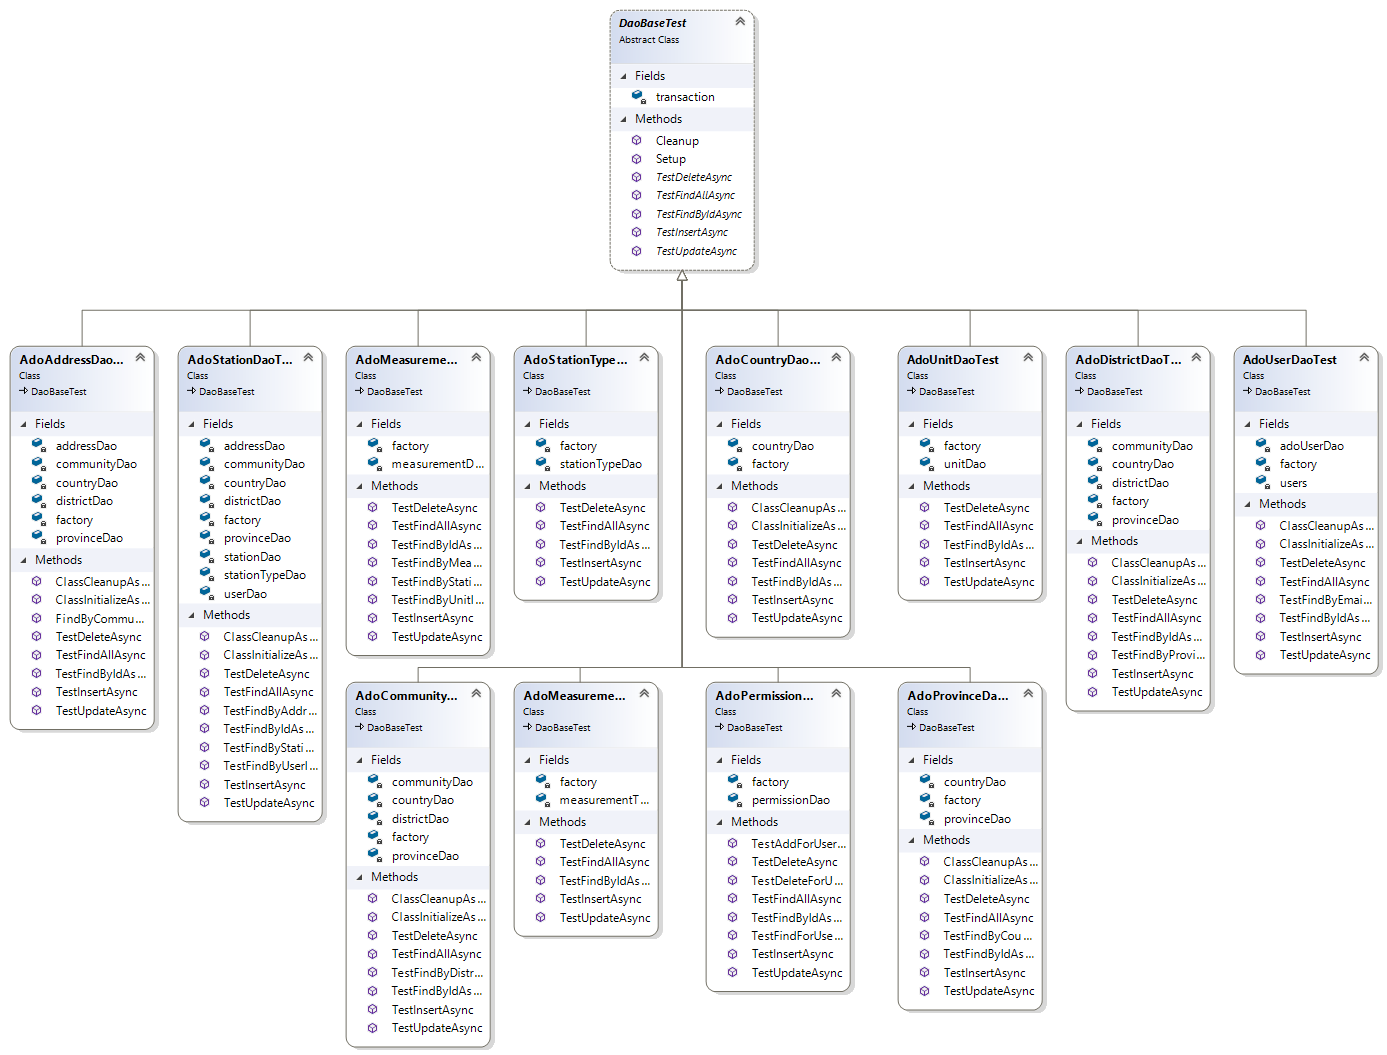
\includegraphics[width=.8\textwidth]{pictures/Wetr_Test_Dal.png}
\caption{Wetr.Domain UML Diagramm}
\label{fig:Wetr.Test.Dal}
\end{figure}
\raggedright

\begin{figure}[H]
\centering
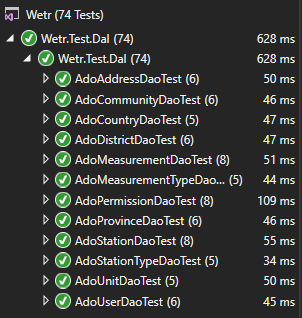
\includegraphics[width=.4\textwidth]{pictures/green_tests.png}
\caption{Beweis, dass die UnitTests erfolgreich durchlaufen.}
\label{fig:Wetr.Test.Dal}
\end{figure}
\raggedright

\newpage
\subsection{Wetr.Generator}
\label{sec:generator}

Der Generator generiert pro \textit{MeasurementType} eine eigene Datei, in der sich die generierten Messdaten befinden. Pro Typ werden nicht genau gleich viele Messdaten generiert, somit ergibt sich eine Summe von etwa 1.2 Millionen Messdaten. Das Format der erzeugten Dateien ist so gestaltet, damit es mit einem speziellen SQL Befehl mittels Bulk-Insert\footnote{https://stackoverflow.com/questions/14330314/bulk-insert-in-mysql} sehr schnell in die Datenbank aufgenommen werden kann. Die generierten Daten haben einen Zeitstempel, der sich innerhalb von einem Jahr bewegt.~\\~\\ %WTF LaTeX?

\textbf{Temperatur}\\
Es wird jede Stunde ein Messwert generiert, der je nach Jahreszeit die Temperatur nach natürlichem Verlauf, sprich zur Mittagszeit ist es am wärmste und in der Nacht am kältesten, gestaltet. Die Werte beinhalten eine zufällige Abweichung von $\pm 1.25$. Der Minimal- bzw. Maximalwert wird pro Jahreszeit nach klimatabelle.info festgelegt.~\\~\\ %WTF LaTeX?

\textbf{Luftfeuchtigkeit}\\
Die Berechnung der Luftfeuchtigkeit funktioniert gleich, wie die der Temperatur, nur, dass die durchschnittlichen Luftfeuchtigkeitswerte hergenommen wurden. Als zufällige Abweichung wurden $\pm10\%$ gewählt.~\\~\\ %WTF LaTeX?

\textbf{Niederschlag}\\
Da nur der jährliche Durchschnittsniederschlag pro Jahreszeit zur Verfügung stand, wurden nicht stündlich, sondern täglich ein Messert generiert. Dieser Wert bewegt sich zwischen $0$ und der Anzahl des durchschnittlichen Tagesniederschalag Mal zwei.~\\~\\ %WTF LaTeX?

\textbf{Luftdruck}\\
Jede Stunde wird ein Luftdruckwert generiert, der zufällig zwischen $900$ und $1100$ Hektopascal liegt.~\\~\\ %WTF LaTeX?

\textbf{Windrichtung}\\
Die Windrichtung ändert sich in dieser einfachen Simulation jede Stunde und kann von $0$ bis $360$ Grad betragen.~\\~\\ %WTF LaTeX?

\textbf{Windstärke}\\
Die Generierung der Windstärke ist in der aktuellen Ausbaustufe sehr primitiv gehalten und ändert sich stündlich zufällig von $0$ und $20\ km/h$
